\documentclass[10pt]{article}
\usepackage[utf8]{inputenc}
\usepackage[spanish]{babel}
\usepackage{amsmath}
\usepackage{amsfonts}
\usepackage{amssymb}
\usepackage{graphics}
\usepackage{graphicx}
\usepackage[left=2cm,right=2cm,top=2cm,bottom=2cm]{geometry}
\usepackage{imakeidx}
\makeindex[columns=3, title=Alphabetical Index, intoc]
\usepackage{listings}
\usepackage{multicol}
\usepackage{changepage}
\usepackage{float}
\usepackage{cite}
\usepackage{url}
\usepackage{hyperref}
\usepackage{pdflscape}
\usepackage[document]{ragged2e}
\usepackage{xcolor,colortbl}
\usepackage{pgf,pgffor}

\hypersetup{
    colorlinks=true,
    linkcolor=blue,
    filecolor=magenta,
    urlcolor=blue,
}

\definecolor{Red}{rgb}{0.7,0,0}
\definecolor{LightCyan}{rgb}{0.88,1,1}
\definecolor{AquaCyan}{rgb}{0.2,1,0.5}
\definecolor{Gray}{gray}{0.85}
\definecolor{DarkBlue}{rgb}{0.1,0.1,0.5}

\definecolor{codegreen}{rgb}{0,0.6,0}
\definecolor{codegray}{rgb}{0.5,0.5,0.5}
\definecolor{codepurple}{rgb}{0.58,0,0.82}
\definecolor{backcolour}{rgb}{0.95,0.95,0.92}

\lstdefinestyle{mystyle}{
    backgroundcolor=\color{backcolour},
    commentstyle=\color{codegreen},
    keywordstyle=\color{magenta},
    numberstyle=\tiny\color{codegray},
    stringstyle=\color{codepurple},
    basicstyle=\ttfamily\footnotesize,
    breakatwhitespace=false,
    breaklines=true,
    captionpos=b,
    keepspaces=true,
    numbers=left,
    numbersep=5pt,
    showspaces=false,
    showstringspaces=false,
    showtabs=false,
    tabsize=3
}
\def\fillandplacepagenumber{%
 \par\pagestyle{empty}%
 \vbox to 0pt{\vss}\vfill
 \vbox to 0pt{\baselineskip0pt
   \hbox to\linewidth{\hss}%
   \baselineskip\footskip
   \hbox to\linewidth{%
     \hfil\thepage\hfil}\vss}}
\lstset{style=mystyle}

\colorlet{punct}{red!60!black}
\definecolor{background}{HTML}{EEEEEE}
\definecolor{delim}{RGB}{20,105,176}
\colorlet{numb}{magenta!60!black}

\lstdefinelanguage{json}{
    basicstyle=\normalfont\ttfamily,
    numbers=left,
    numberstyle=\scriptsize,
    stepnumber=1,
    numbersep=8pt,
    showstringspaces=false,
    breaklines=true,
    frame=lines,
    backgroundcolor=\color{background},
    literate=
     *{0}{{{\color{numb}0}}}{1}
      {1}{{{\color{numb}1}}}{1}
      {2}{{{\color{numb}2}}}{1}
      {3}{{{\color{numb}3}}}{1}
      {4}{{{\color{numb}4}}}{1}
      {5}{{{\color{numb}5}}}{1}
      {6}{{{\color{numb}6}}}{1}
      {7}{{{\color{numb}7}}}{1}
      {8}{{{\color{numb}8}}}{1}
      {9}{{{\color{numb}9}}}{1}
      {:}{{{\color{punct}{:}}}}{1}
      {,}{{{\color{punct}{,}}}}{1}
      {\{}{{{\color{delim}{\{}}}}{1}
      {\}}{{{\color{delim}{\}}}}}{1}
      {[}{{{\color{delim}{[}}}}{1}
      {]}{{{\color{delim}{]}}}}{1},
}

\title{Introducción a bases de datos\\Sesión 5}

\author{Adrian González Pardo}

\date{\today}

\newcommand\tab[1][1cm]{\hspace*{#1}}

\begin{document}
\maketitle
\section{Ejemplos}
\subsection{Ejemplo 1}
\begin{center}
  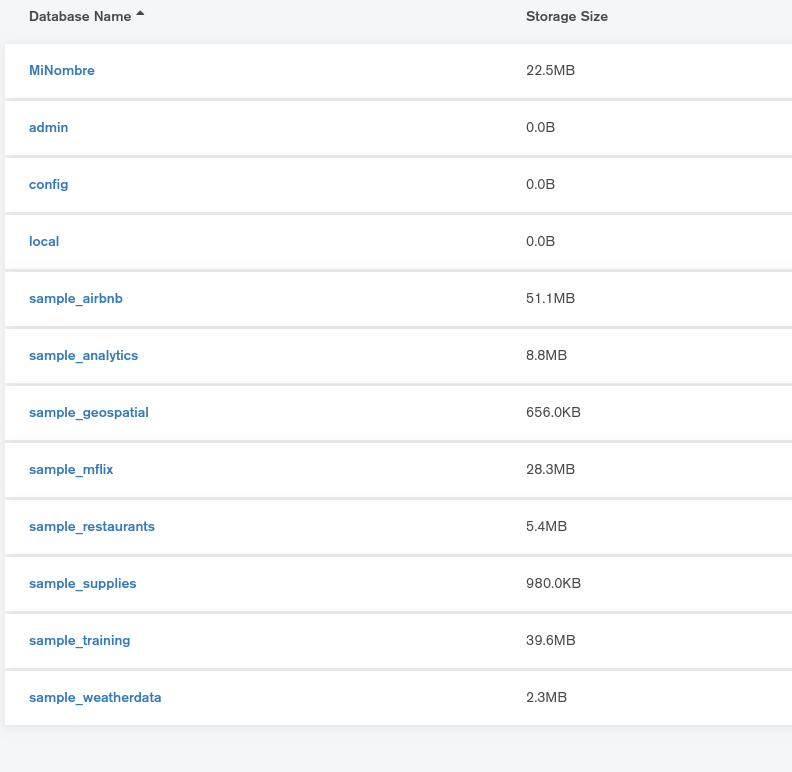
\includegraphics[scale=0.35]{imgs/ej1_1.png}\\
  \textit{Carga de nuevas bases de datos y colecciones de datos de ejemplo del mismo MongoDB Cluster}\\
  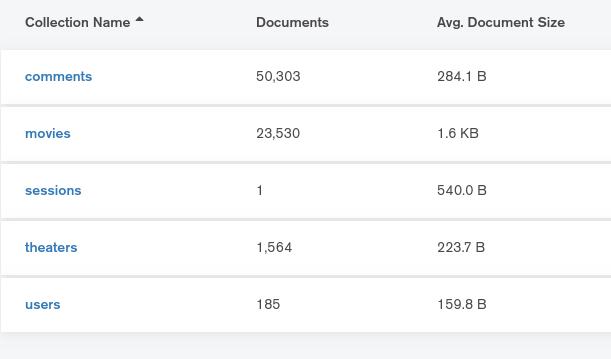
\includegraphics[scale=0.35]{imgs/ej1_2.png}\\
  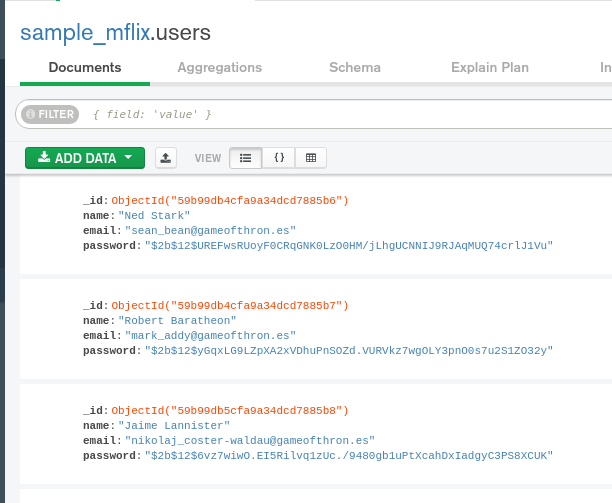
\includegraphics[scale=0.35]{imgs/ej1_3.png}\\
  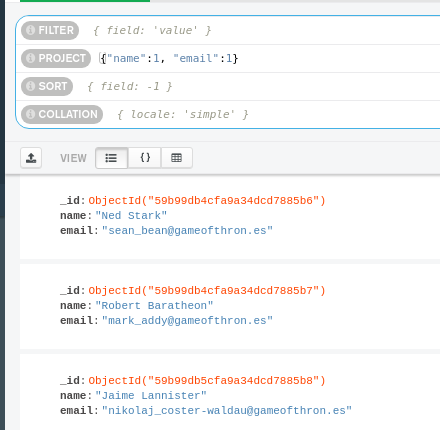
\includegraphics[scale=0.35]{imgs/ej1_4.png}\\
  \textit{Consulta/Proyeccion de la colección users de mflix}

\end{center}
\subsection{Ejemplo 2}
\begin{center}
  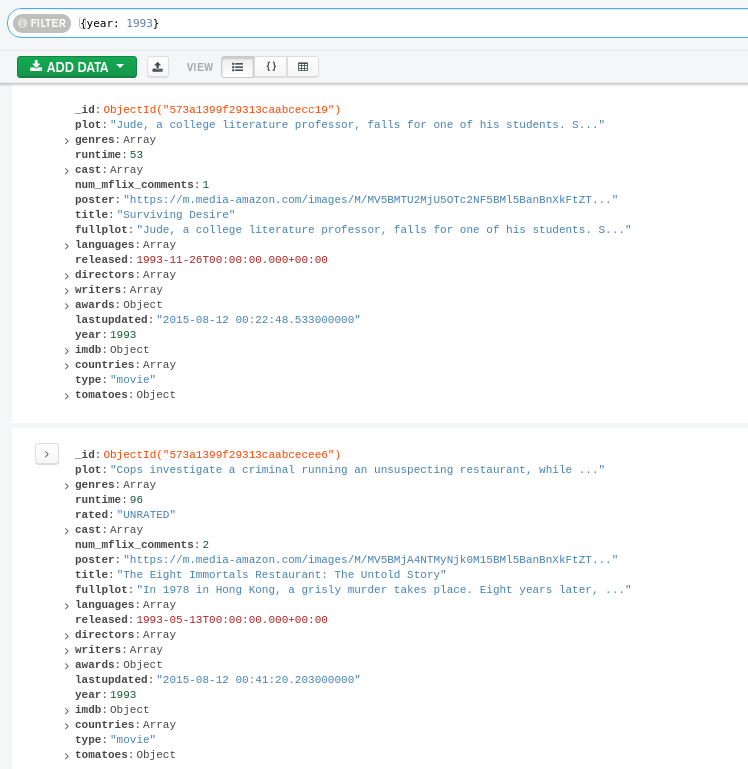
\includegraphics[scale=0.35]{imgs/ej2_1.png}\\
  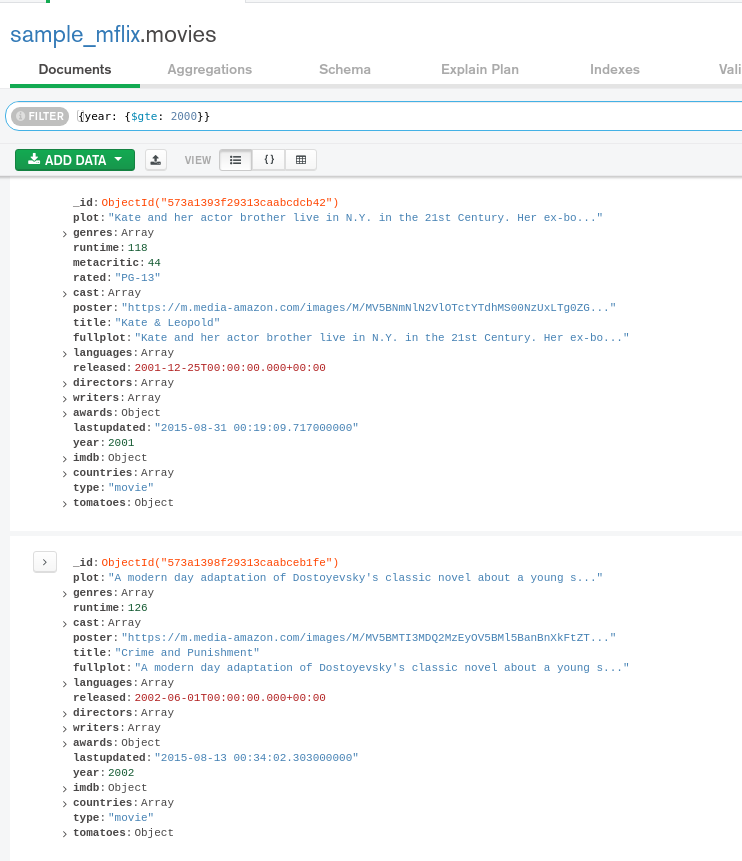
\includegraphics[scale=0.35]{imgs/ej2_2.png}\\
  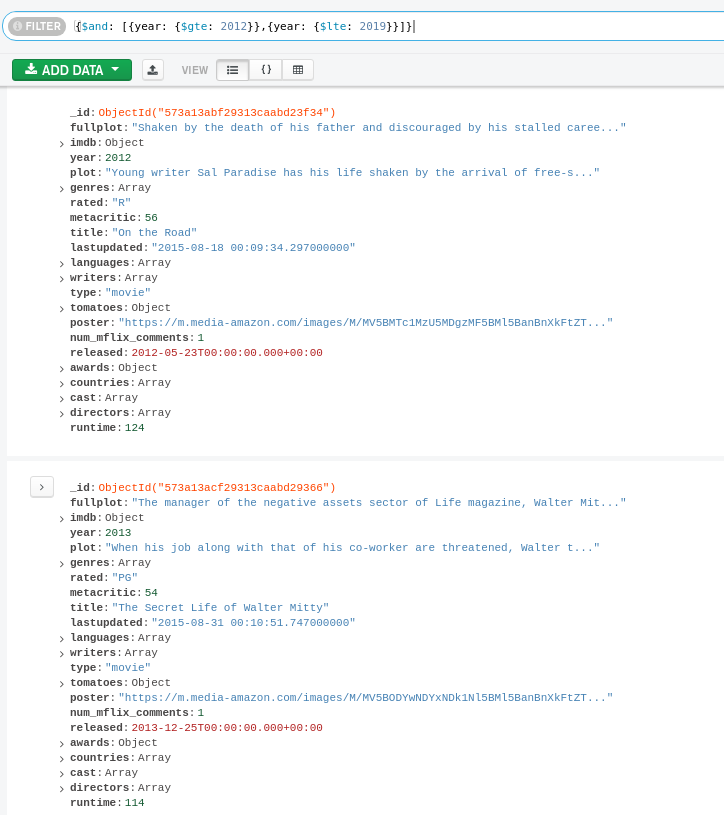
\includegraphics[scale=0.35]{imgs/ej2_3.png}\\
  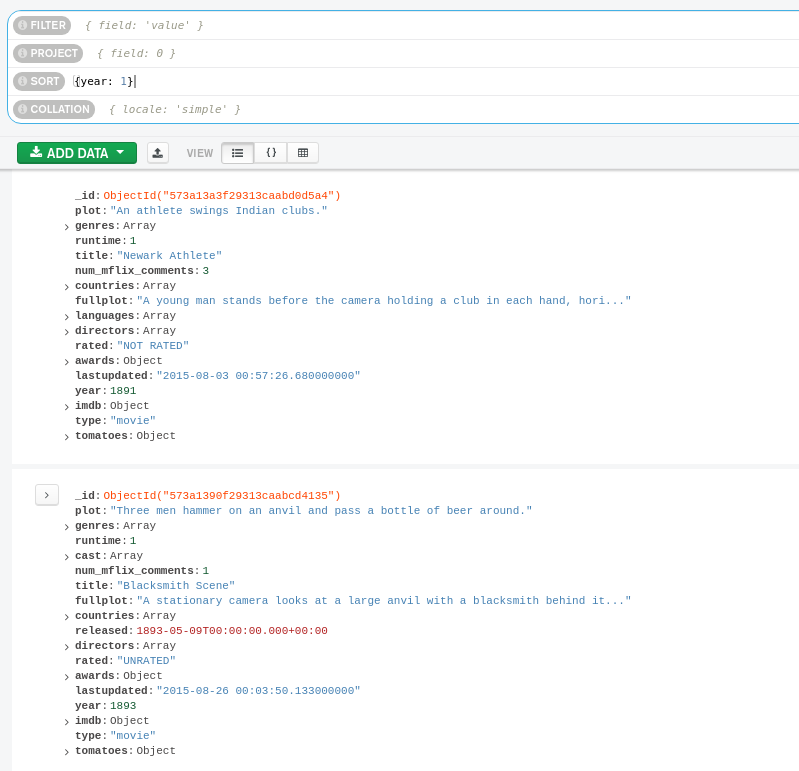
\includegraphics[scale=0.35]{imgs/ej2_4.png}\\
  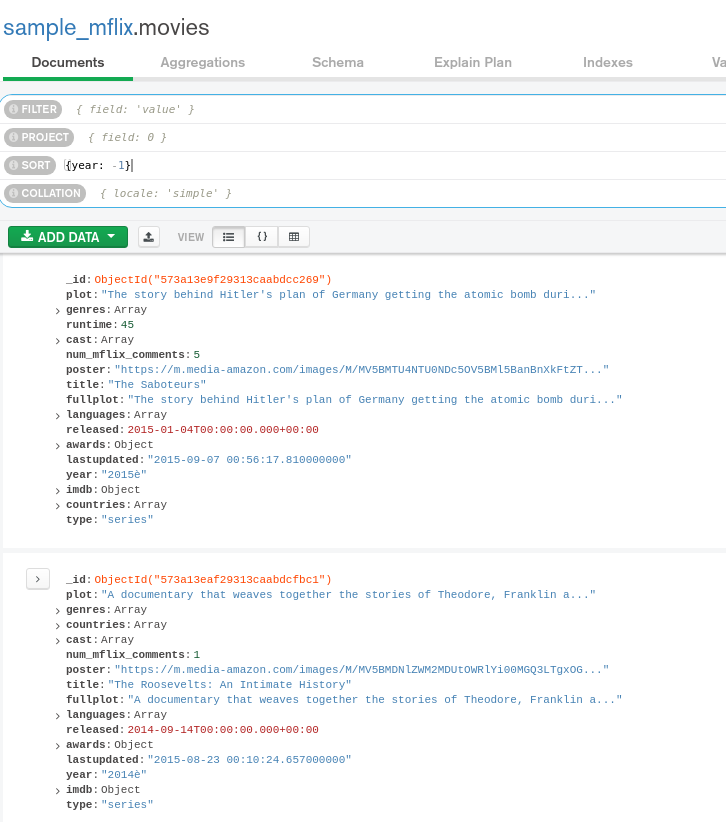
\includegraphics[scale=0.35]{imgs/ej2_5.png}\\
  \textit{Filtros y ordenamiento}
\end{center}
\clearpage
\section{Retos}
\subsection{Reto 1}
\begin{center}
  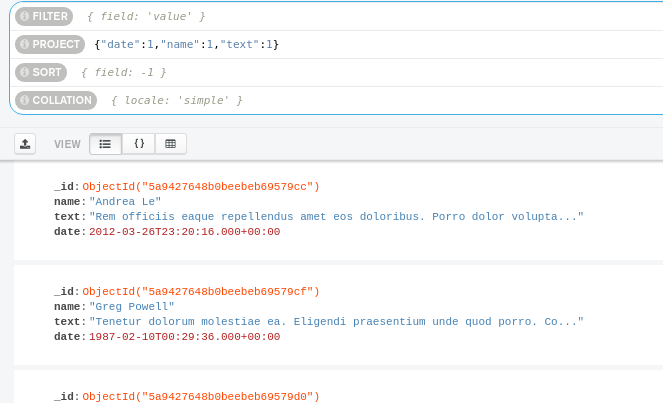
\includegraphics[scale=0.35]{imgs/e1_1.png}\\
  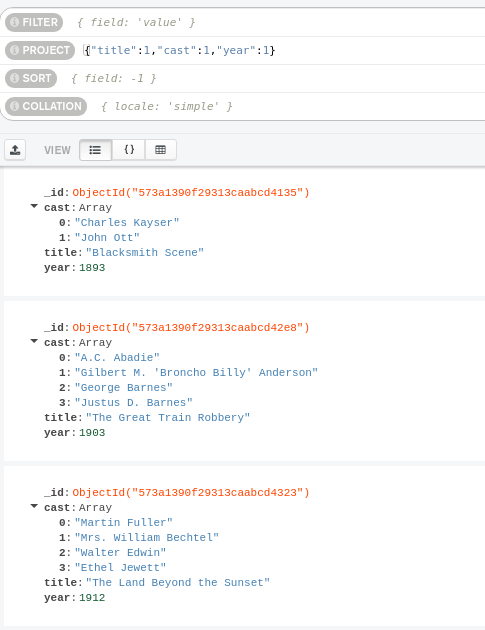
\includegraphics[scale=0.35]{imgs/e1_2.png}\\
  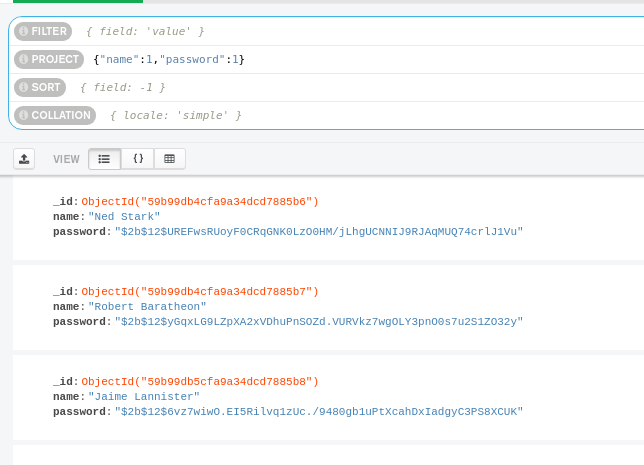
\includegraphics[scale=0.35]{imgs/e1_3.png}\\
  \textit{Consulta/Proyeccion de la colección users de mflix}
\end{center}
\subsection{Reto 2}
\begin{center}
  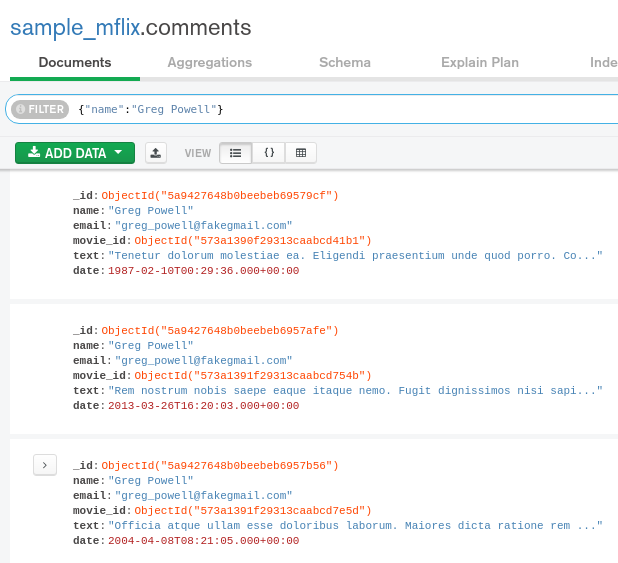
\includegraphics[scale=0.35]{imgs/e2_1.png}\\
  \textit{Filtro de comentarios hechos por Greg Powell}\\
  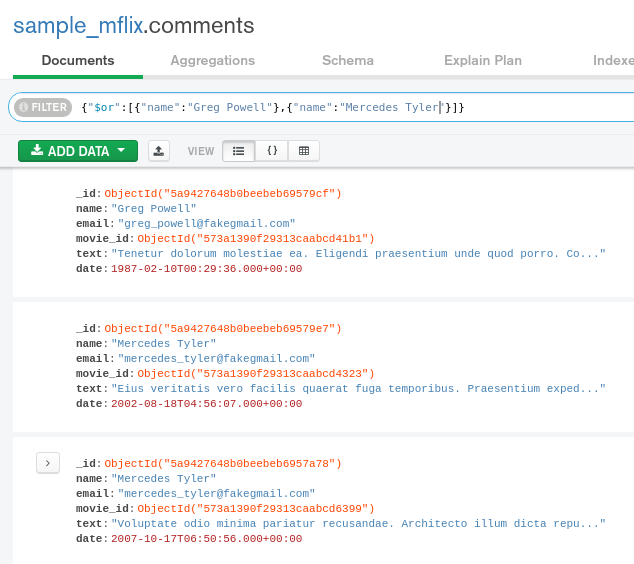
\includegraphics[scale=0.35]{imgs/e2_2.png}\\
  \textit{Filtro de comentarios hechos por Greg Powell o Mercedes Tyler}\\
  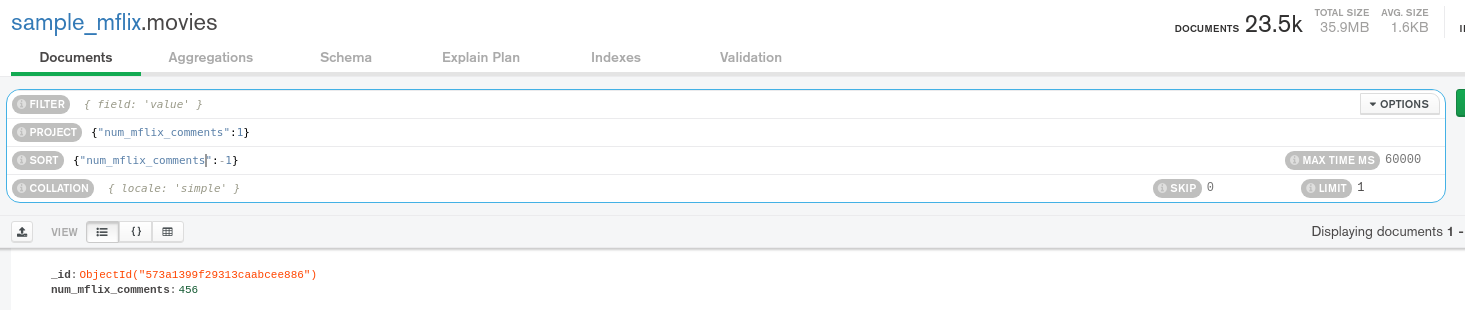
\includegraphics[scale=0.35]{imgs/e2_3.png}\\
  \textit{Muestra el máximo número de comentarios en una película}\\
  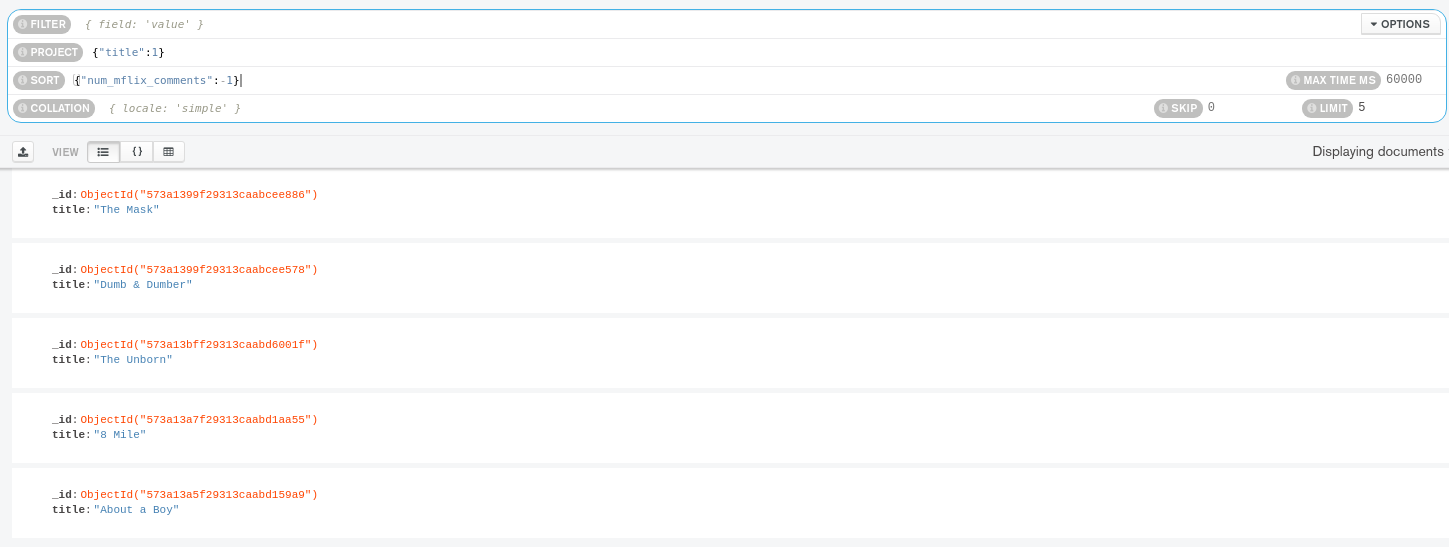
\includegraphics[scale=0.35]{imgs/e2_4.png}\\
  \textit{Muestra el título de las cinco películas más comentadas}
\end{center}
\clearpage
\section{Ejercicio}
\begin{center}
  \foreach \x [count=\xi] in {1,...,13}{
    \includegraphics[scale=0.35]{imgs/ex_\xi.png}\\
    \textit{Ejercicio 1 inciso \xi}\\
  }
  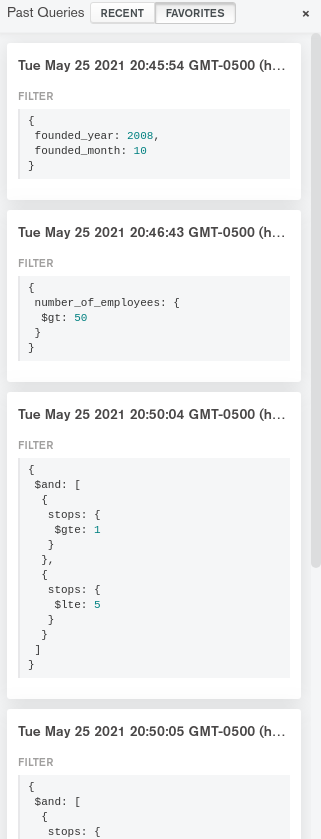
\includegraphics[scale=0.35]{imgs/ex_final.png}\\
  \textit{Ejercicio captura de queries favoritos}
\end{center}
\lstinputlisting[language=json]{ejercicio.json}
\end{document}
